\documentclass[12pt]{report}
\usepackage{enumitem}
\usepackage{longtable}

\usepackage{tikz}
\usetikzlibrary{shapes, arrows, positioning}


\usepackage{booktabs}

\usepackage{titlesec}
\usepackage{subcaption}
\usepackage[labelformat=parens,labelsep=quad,skip=3pt]{caption}
\setcounter{secnumdepth}{4}

\usepackage[justification=centering]{caption}

\usepackage{array,multirow,graphicx}
\usepackage{bigstrut}

\usepackage[most]{tcolorbox}

\usepackage{amsmath}
\usepackage{hyperref}
\hypersetup{
    colorlinks,
    citecolor=black,
    filecolor=black,
    linkcolor=black,
    urlcolor=black
}

\usepackage{fullpage}
\usepackage{setspace}
\usepackage{fancyhdr}
\usepackage{acronym} 

\pagestyle{fancy}
\fancyhf{}
\rhead{\rightmark}
% \lhead{\leftmark}
% \lhead{\thechapter}
% \lhead{\small\leftmark}
\rfoot{\thepage}
\renewcommand{\baselinestretch}{1.1}

\setlength{\parindent}{2em}
\setlength{\parskip}{0.5em}
\setlength{\headsep}{15mm}
\usepackage{float}
\graphicspath{{chapters/sprint1/}{chapters/sprint2/}{chapters/sprint3/}{chapters/sprint4/}{chapters/sprint5/}}
\usepackage[T1]{fontenc}

\usepackage{xcolor}
\usepackage{tabularx}
\usepackage{pifont}
\fancypagestyle{noheader}{
  \fancyhf{}% Clear header/footer
  \renewcommand{\headrulewidth}{0pt}% No header rule
}

\newlist{negitemize}{itemize}{1}
\setlist[negitemize,1]{label=\ding{56}} % \ding{56} is the ✕ symbol in pifont

\newlist{positemize}{itemize}{1}
\setlist[positemize,1]{label=\ding{51}}

\begin{document}
\renewcommand\bibname{References}

\pagenumbering{gobble}

\chapter*{Dedication}
\vspace*{2cm}
\begin{center}
This humble effort is dedicated to \bigbreak  Mom, Dad, family and friends..
\end{center}
\chapter*{Acknowledgment}

First of all, I humbly thank God Almighty, the Merciful and Beneficent, who granted us health, wisdom, and supportive people, enabling me to achieve this goal.
\\

I heartily thank my academic supervisor, Mr. Abderrazek Hachani, whose encouragement, guidance, and support from the initial to the final stages enabled me to develop an understanding of the project.
\\

Furthermore, I would like to acknowledge with much appreciation the crucial role of my supervisor, Mr. Abdelhamid Jemma, who contributed significantly to this project through close supervision, important suggestions, encouragement, and patience.
\\

I am grateful to all my professors for their support in numerous ways. They sincerely guided us and provided services for every activity and task that boosted our self-esteem and taught us to be more responsible for our own good and for others.
\\

Last but not least, Special thanks also go to my close friends, Yosra and Mawahebb, whose unwavering support and encouragement kept me motivated throughout this journey.

% \newpage
\pagestyle{empty}
\section*{Acronym List}  % Section title without numbering
\addcontentsline{toc}{section}{Acronyms} % Add acronyms to the table of contents
\begin{acronym}
  \acro{API}{Application Programming Interface}
  \acro{CI/CD}{Continuous Integration/Continuous Deployment}
  \acro{K8s}{Kubernetes}
  \acro{REST}{Representational State Transfer}
\end{acronym}


\tableofcontents
\listoffigures
\listoftables

\newpage

\chapter*{General Introduction}
In today’s fast-evolving technological landscape, businesses increasingly need to leverage multiple cloud service providers to maintain flexibility, reduce costs, and avoid vendor lock-in. This shift has significantly increased the operational complexity of managing resources and services across various cloud platforms. As a result, the demand for a unified management solution has become more critical for companies aiming to streamline their operations and optimize their IT infrastructure.

Ilef Export, a prominent player in Tunisia's agricultural export industry, recognizes the strategic importance of integrating advanced IT solutions to enhance operational efficiency and competitiveness. To support this vision, Ilef Export is establishing a robust IT department to drive innovation and support the company’s growth objectives. My final year project aligns with this initiative, aiming to develop a unified platform that efficiently manages resources and services across multiple cloud providers, including AWS, Google Cloud, and Azure.

The project's primary goal is to design and implement a comprehensive solution that addresses the challenges of multi-cloud management. This involves overcoming operational complexities, mitigating the risks of vendor lock-in, and optimizing cost management. The platform will facilitate the creation of Docker images, deploying them to a private registry, and subsequently deploying them to a server. Additionally, integrating a Nexus repository registry will enhance artifact management within the development lifecycle.

This project aims not only to provide Ilef Export with state-of-the-art IT infrastructure but also to lay the foundation for future technological advancements. By successfully completing this project, Ilef Export will be well-positioned to harness the full potential of cloud technologies, driving innovation, improving productivity, and ensuring sustainable growth in the competitive agricultural export market.

The following sections of this report will delve into the detailed methodologies, design considerations, implementation strategies, and the results of this project. This comprehensive exploration aims to demonstrate how the proposed unified platform can address the outlined challenges and objectives effectively.\thispagestyle{noheader}
\cleardoublepage

\clearpage
\cleardoublepage% ensures that the page numbering will change on a recto page
\pagenumbering{arabic}


\chapter{Overview}

In this chapter, we will provide a thorough overview of the project. We will begin by discussing the general context, covering both the educational and professional backgrounds. Next, we will detail the project itself, identifying the problem, reviewing existing solutions, and presenting our innovative approach. Lastly, we will describe the methodology used in the project, including the team structure and roles. This structured approach will ensure a comprehensive understanding of the project's scope, objectives, and implementation strategy.

\pagebreak

\section{General context}
This part is dedicated to present the project context such as the scholar and the professional frame.

\subsection{Pedagogical frame}

This project was undertaken as part of a graduation internship, the final step in obtaining an engineering degree in computer science from the Private Higher School of Engineering and Technology "ESPRIT" \hyperref[fig:ilef_logo]{(Logo: Figure \ref{fig:esprit_logo})}.
 The internship spanned six months, from January 1st to July 1st, 2024, during which I integrated with the development team at Ilef Export.
 

\begin{figure}[htbp]
  \centering  % Add this line to center the image
  \includegraphics[width=12cm]{./chapters/overview/esprit.jpeg}
  \caption{ESPRIT logo}
  \label{fig:esprit_logo}
\end{figure}

\subsection{Professional frame}
% \vspace*{64pt}

Ilef Export \hyperref[fig:ilef_logo]{(Logo: Figure \ref{fig:ilef_logo})} is a prominent Tunisian company headquartered in Tunisia. Specializing in the export of high-quality dates and vegetables, Ilef Export has established itself as a key player in the agricultural export industry. Founded with a commitment to excellence, the company has built a strong reputation for delivering premium products to its clients.

Ilef Export serves a range of distinguished clients, including Monoprix, and focuses its export efforts primarily on markets in Morocco, France, and Canada... The company's strategy is centered on maintaining stringent quality standards, ensuring exceptional customer satisfaction, and continuously expanding its market presence.
Through its dedication to quality and innovation, Ilef Export aims to solidify its position as a leader in the global agricultural export sector.

\begin{figure}[htbp]
  \centering  % Add this line to center the image
  \includegraphics[width=8cm]{./chapters/overview/ilef_logo.png}
  \caption{ILEF Export logo}
  \label{fig:ilef_logo}
\end{figure}



\section{Project presentation}
\subsection{Problematic}
Ilef Export, a leading exporter in Tunisia specializing in dates and vegetables, maintains a prominent presence in global markets such as Morocco, France, and Canada. However, the company faces several significant challenges in its cloud operations:

\begin{itemize}
  \item \textbf{Complex Management }:
  Managing services across multiple cloud providers (AWS, Google Cloud, Azure, and Hetzner) is complicated due to different tools and processes. This complexity leads to inefficiencies and increased operational costs.

  \item \textbf{Vendor Lock-In }:
  Relying on a single cloud provider creates a risk of vendor lock-in, making it difficult to switch or balance workloads across providers. This dependency limits flexibility and can potentially increase costs.

  \item \textbf{Time Inefficiencies }:
  Setting up instances/clusters and deploying Docker containers across various cloud providers takes a significant amount of time, causing delays in deployment and impacting overall productivity.

  \item \textbf{Cost Control }:
  Tracking and managing costs across different cloud providers is challenging, leading to unpredictable expenses and budget issues.

  \item \textbf{Lack of Unified Management }:
  Without a single platform to manage all cloud services efficiently, the teams face fragmented processes and poor resource utilization.
\end{itemize}


\subsection{Examination of current solutions}
To address the challenges in managing multi-cloud environments, it is crucial to examine existing solutions and their limitations. This evaluation will focus on three popular multi-cloud management platforms: \textbf{ Flexera} (formerly RightScale), \textbf{CloudBolt}, and \textbf{CloudHealth}.
\subsubsection{Flexera}
\begin{itemize}
  \begin{figure}[htbp]
    \centering  % Add this line to center the image
    \includegraphics[width=5cm]{./chapters/overview/flexera.jpg}
    \caption{Flexera logo}
    \label{fig:flexera}
  \end{figure}
  \item \textbf{Capabilities }:
Flexera provides a unified interface for managing multiple cloud environments, including AWS, Google Cloud. It offers features for cloud cost management, automated workflows, and governance.

\item \textbf{Limitations }:
\begin{negitemize}
  \item \textbf{Cost }: Flexera can be expensive, particularly for small to medium-sized enterprises. The pricing model can become a significant burden as the scale of cloud operations increases.
  \item \textbf{Complexity }: The initial setup and configuration of Flexera can be complex and time-consuming, requiring specialized knowledge and resources.
\end{negitemize}
\end{itemize}


\subsubsection{CloudBolt}

\begin{figure}[htbp]
  \centering  % Add this line to center the image
  \includegraphics[width=4cm]{./chapters/overview/cloudbolt.jpg}
  \caption{Cloudbolt logo}
  \label{fig:cloudbolt}
\end{figure}

\begin{itemize}
  \item \textbf{Capabilities }:
  CloudBolt offers comprehensive multi-cloud management, including provisioning, orchestration, and cost optimization. 
\item \textbf{Limitations }:
\begin{negitemize}
  \item \textbf{User Experience }: The user interface can be less intuitive compared to other platforms, leading to a steeper learning curve for new users.
  \item \textbf{Performance }: Some users have reported performance issues when managing large-scale deployments, which can impact overall efficiency.
\end{negitemize}
\end{itemize}

\subsubsection{CloudHealth}
\begin{figure}[htbp]
  \centering  % Add this line to center the image
  \includegraphics[width=6cm]{./chapters/overview/cloudhealth.png}
  \caption{Cloudhealth logo}
  \label{fig:cloudhealth}
\end{figure}

\begin{itemize}
  \item \textbf{Capabilities }:
  CloudHealth by VMware provides robust cloud cost management, governance, and security features across multiple cloud environments, including AWS, Google Cloud, and Azure.

\item \textbf{Limitations }:
\begin{negitemize}
  \item \textbf{Cost}:  CloudHealth can be relatively expensive, especially for smaller organizations. The pricing structure may become burdensome as cloud usage scales.
  \item \textbf{Provider Support }: CloudHealth does not support many cloud providers such as Hetzner, limiting its usefulness for organizations utilizing this provider.

\end{negitemize}
\end{itemize}

\subsection{The proposed solution}
To address the identified challenges and limitations of existing solutions, Ilef Export proposes the development of a unified platform tailored to its specific needs. This platform will streamline operations, enhance flexibility, and provide better visibility into costs across multiple cloud providers, including AWS, Google Cloud, Azure, and Hetzner.

The proposed solution includes the following key components:
\begin{positemize}
  \item \textbf{ Unified Interface:}
  Develop a single interface to manage virtual machines, containers, and other resources across all supported cloud providers.

  \item \textbf{ Automated Workflows:}
  Develop automated workflows for deploying Docker containers and setting up instances, significantly reducing the time and effort required for these processes.

  \item \textbf{ Cost Visualization: }
  Implement tools to track and visualize cloud costs, providing clear insights into expenses across different providers.

  \item \textbf{ Kubernetes Integration:}
  Include tools for managing Kubernetes clusters, simplifying the deployment and scaling of containerized applications to meet the company's specific needs.
\end{positemize}



\section{Methodology}
The software development process involves a series of tasks that result in the creation of new software or modifications to existing systems. No single process is flawless, and companies often adapt their methodologies based on specific needs, which can vary depending on stakeholders, circumstances, and project characteristics. The primary goal of a development methodology is to enhance the quality of the product. Adopting a project management methodology is crucial for helping team members achieve their goals within set time frames. 
\subsection{Agile Methodologies}
Agile methodology is a project management strategy commonly used in software development. This approach helps teams address the unpredictability of software creation through incremental, iterative work cycles known as sprints. A sprint is a designated time frame for completing a specific phase of a project. Once this period concludes, the sprint is considered finished, regardless of whether all team members agree on the development’s quality. The project continues to evolve in subsequent phases, each adhering to its scheduled duration. Agile emphasizes flexibility, continuous improvement, and collaboration, enabling teams to adapt to changes quickly and deliver high-quality software.
\subsection{Scrum method}
Scrum as shown in the \hyperref[fig:scrum]{(Figure \ref{fig:scrum})} is an iterative and incremental approach within agile software development. In Scrum, the sprint serves as the fundamental development unit. Each sprint begins with a planning session to outline tasks and set goals. At the end of the sprint, a review or retrospective meeting evaluates the progress and identifies lessons for future sprints. Throughout each sprint, the team works on producing completed segments of the product. Scrum promotes transparency, inspection, and adaptation, ensuring that the development process remains efficient and aligned with project goals. The key roles in Scrum include the Product Owner, Scrum Master, and Development Team, each contributing to the successful execution of sprints and overall project delivery.
\vspace{1cm}

Given the iterative changes and evolving requirements of our project, we have chosen the Agile methodology and the Scrum framework to ensure flexibility and continuous improvement.

\vspace{1cm}
\begin{figure}[htbp]
  \centering  % Add this line to center the image
  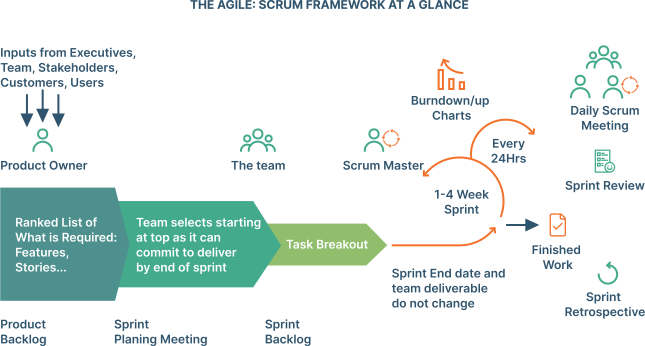
\includegraphics[width=13cm]{./chapters/overview/scrum.png}
  \caption{Scrum process}
  \label{fig:scrum}
\end{figure}

\vspace{1cm}
\subsubsection{Project team}
The table \hyperref[p]{\ref{p}} introduces the project team members and their roles.

\begin{table}[!htbp]
\centering
  \begin{tabular}{ | p{3cm}  | p{6cm} |}
    \hline

    Scrum role    & Name          \\ \hline

    Product owner & Abdelhamid Jemaa  \\ \hline
    Scrum Master  & Chaker Benhamad   \\ \hline
    Team members  & Mehrez Benhamad \\ \hline

    \hline
  \end{tabular}
\caption{Project members and roles}
\label{p}
\end{table}

\section*{Conclusion}
In this chapter, we have offered a detailed overview of the project, beginning with the general context that includes both pedagogical and professional frameworks. We identified the problem, evaluated existing solutions, and presented our innovative approach. Additionally, we outlined the project methodology, including the team composition and their roles. This structured approach has provided a clear understanding of the project's scope, objectives, and execution strategy.

By establishing this solid foundation, we are well-prepared for the subsequent phases of the project, enabling us to achieve our desired outcomes efficiently and effectively.

In the next chapter, "Preliminary Study," we will delve deeper into the initial research and analysis conducted to inform our project's direction.
% \chapter{State of the Art}

This chapter delves into the critical concepts and definitions pivotal to understanding the landscape of our project. We explore the fundamental technologies and methodologies that drive our development process, focusing on Cloud Computing, Software as a Service (SaaS), and other key areas such as software provisioning, scalability, containerization, serverless computing, and REST architecture. Each section aims to provide a comprehensive overview of these concepts, emphasizing their relevance and application within our project's framework.

Additionally, we will address challenges such as vendor lock-in and discuss strategic approaches like orchestration and agile methodologies, which are essential for managing modern software projects efficiently. Through this exploration, we establish a solid foundation of knowledge that supports the advanced functionalities of our platform.

\pagebreak

\section{Cloud}
Cloud computing refers to an Internet-driven approach that delivers shared computing resources and data services to various devices as required. It is designed to provide ubiquitous, on-demand access to a collection of configurable computing resources (including networks, servers, storage, applications, and services) that can be quickly allocated and deallocated with minimal management effort. These cloud services offer both individuals and businesses the ability to store and manage data in data centers that are either privately operated or owned by third parties, which could be situated locally or internationally. The concept of cloud computing depends on resource sharing to maintain consistency and cost efficiency, akin to the operation of utilities such as the electrical grid.


\section{SaaS}
Software as a Service (SaaS) is a cloud computing model where software applications are hosted by a third-party provider and made available to customers over the internet. Users can access these applications via a web browser, eliminating the need to install or maintain software locally on their devices. This model offers convenience, scalability, and cost-effectiveness for both individual users and organizations.

\section{Software provisioning}
Software provisioning refers to the process of preparing and equipping a computer system with necessary software applications and configurations to fulfill specific operational requirements. It involves tasks such as installation, configuration, and initial setup of software components needed to support business operations or user requirements within an IT environment.


\section{Scalability}
Scalability refers to the capability of a system, network,
or process to handle a growing amount of work or its potential to be enlarged
to accommodate that growth. It is an essential characteristic for systems that are expected to expand over time.
Scalability can be vertical or horizontal:

$\bullet$ \textbf{Vertical Scalability (Scaling Up)}: This involves adding more power (such as CPU, RAM) to an existing machine. It means enhancing the capacity of a single resource.

$\bullet$ \textbf{Horizontal Scalability (Scaling Out)}: This involves adding more machines or devices to a system so that the workload and processing power are distributed across multiple units.

In the context of computing and business applications, scalability ensures that the system can maintain or improve its performance and efficiency as the demand for resources or services increases. It is a critical factor in the design and architecture of applications, especially those that require handling large volumes of data or high user traffic.

\section{ Containerization}
Containerization is a lightweight form of virtualization that involves
encapsulating an application and its dependencies into a container. 
This container is a standardized unit of software that packages up the code and all its dependencies so the application runs quickly and reliably from one computing environment to another.

\section{Serverless computing}
Serverless computing, also referred to as Function as a Service (FaaS), is a cloud computing model in which the cloud provider takes care of the infrastructure required to run code. This allows developers to concentrate on creating and deploying specific functions or segments of business logic without the need to manage servers or hardware.


\section{REST architecture}
REST, which stands for Representational State Transfer, is an architectural style used for designing networked applications. It facilitates the creation and modification of resources with ease, serving as a lightweight alternative to complex mechanisms such as RPC, CORBA, and SOAP.

REST is not a formal standard but a set of guidelines for building efficient communication frameworks between two machines using the HTTP protocol. The World Wide Web, which operates over HTTP, can be seen as a prime example of a REST-based architecture. REST utilizes a stateless, client-server, cacheable communication protocol, making it simple to implement and maintain. Furthermore, it enhances scalability by supporting multiple backend services simultaneously.

Similar to web services, a REST service is platform-independent and language-independent, operating over HTTP and functioning effectively even behind firewalls.

There are several fundamental concepts that distinguish REST from other web services. These key principles include:

$\bullet$ \textbf{Unique URL-Resource mapping}: Each resource is associated with a unique URL, providing a logical way to access specific information. 

$\bullet$ \textbf{Statelessness}: All information required to process a request is included within the request itself, meaning the server does not retain any state from previous requests. This principle is derived from the stateless nature of HTTP.

$\bullet$ \textbf{Action Verbs}: REST uses HTTP verbs to specify the action to be performed. The primary HTTP verbs in REST architecture are GET, POST, PUT, and DELETE. GET retrieves resources, PUT updates resources, POST creates new resources, and DELETE removes resources.

$\bullet$ \textbf{Data Exchange formats}: REST does not mandate a specific data encoding format for resource bodies. Common formats include JSON \cite{json} and XML, but others like PROTOBUF and YAML are also supported.


% \subsection{Numeric Metrics}
% \begin{itemize}
%     \item \textbf{Accuracy}: We report class-wise accuracy by considering True Positive (TP) as the positive reviews which were
% correctly predicted as positive, and True Negative (TN) as those reviews which were correctly classi-
% fied as negative. Then, False Positives (FP) and False Negatives (FN) follow intuitively. The actual
% accuracy of the models were obtained with Equation \ref{eq1}.

% \begin{equation} \label{eq1}
% Accuracy = \frac{TP+TN}{TP+FP+TN+FN}
% \end{equation}
%     \item \textbf{True Positive Rate/Recall/Hit Rate/Sensitivity}: The true positive rate (TPR) measures the proportion of correctly identified actual positives (TP).

% \begin{equation} \label{eq1}
% TPR = \frac{TP}{TP+FN} = 1 - False Negative Rate
% \end{equation}
% \item \textbf{ False Positive Rate/Fall-Out } : The false positive rate (FPR) measures the proportion of incorrectly identified actual negatives (FP).
% \begin{equation} \label{eq1}
% FPR = \frac{FP}{FP+TN} = 1 - Specificity
% \end{equation}

% \end{itemize}



% \subsection{Vendor lock-in}
\section{Vendor lock-in}

Vendor lock-in is a situation where a customer becomes dependent on a specific vendor for products and services,
making it difficult to switch to another provider without incurring significant costs, inconvenience,
or compatibility issues. This dependency can arise from various factors such as proprietary technologies,
unique data formats, or specific software that are incompatible with other vendors' systems.
Vendor lock-in can lead to reduced flexibility, higher costs, and increased risk for the customer,
as they may struggle to adapt to new technologies or negotiate better terms. To mitigate vendor lock-in, organizations can adopt open standards, ensure data portability, negotiate flexible contracts, and diversify their technology stack across multiple vendors.


\section{Orchestration}
Orchestration in computing refers to the automated arrangement, coordination, and management of complex computer systems, middleware, and services. It involves organizing multiple automated tasks and workflows to ensure they function together seamlessly, often in cloud environments, containers, and microservices architectures. Orchestration tools streamline and simplify the deployment, scaling, and operations of applications, enabling efficient resource use, consistency, and scalability.




% \section{Agile}

\section*{Conclusion}
In this chapter, we introduced general concepts and general approaches
used in this project. Also, we have presented the problematic of our project and existing tools condiatate to solve it.

\chapter{Preliminary study}

Building on the foundational definitions and technical frameworks previously discussed, this chapter offers an in-depth overview of our project, the Ilef Unified Cloud Management Platform. We start by examining the requirements to outline the essential functional and non-functional specifications critical for the platform’s design and implementation. Next, we will construct the Product Backlog to steer our project goals. Lastly, we will illustrate the primary use cases for the platform, highlighting its capability to enable efficient management and interoperability among various cloud providers and services.


\pagebreak

\section{Basic concepts}

\section{Cloud}
Cloud computing refers to an Internet-driven approach that delivers shared computing resources and data services to various devices as required. It is designed to provide ubiquitous, on-demand access to a collection of configurable computing resources (including networks, servers, storage, applications, and services) that can be quickly allocated and deallocated with minimal management effort. These cloud services offer both individuals and businesses the ability to store and manage data in data centers that are either privately operated or owned by third parties, which could be situated locally or internationally. The concept of cloud computing depends on resource sharing to maintain consistency and cost efficiency, akin to the operation of utilities such as the electrical grid.


\section{SaaS}
Software as a Service (SaaS) is a cloud computing model where software applications are hosted by a third-party provider and made available to customers over the internet. Users can access these applications via a web browser, eliminating the need to install or maintain software locally on their devices. This model offers convenience, scalability, and cost-effectiveness for both individual users and organizations.

\section{Software provisioning}
Software provisioning refers to the process of preparing and equipping a computer system with necessary software applications and configurations to fulfill specific operational requirements. It involves tasks such as installation, configuration, and initial setup of software components needed to support business operations or user requirements within an IT environment.


\section{Scalability}
Scalability refers to the capability of a system, network,
or process to handle a growing amount of work or its potential to be enlarged
to accommodate that growth. It is an essential characteristic for systems that are expected to expand over time.
Scalability can be vertical or horizontal:

$\bullet$ \textbf{Vertical Scalability (Scaling Up)}: This involves adding more power (such as CPU, RAM) to an existing machine. It means enhancing the capacity of a single resource.

$\bullet$ \textbf{Horizontal Scalability (Scaling Out)}: This involves adding more machines or devices to a system so that the workload and processing power are distributed across multiple units.

In the context of computing and business applications, scalability ensures that the system can maintain or improve its performance and efficiency as the demand for resources or services increases. It is a critical factor in the design and architecture of applications, especially those that require handling large volumes of data or high user traffic.

\section{ Containerization}
Containerization is a lightweight form of virtualization that involves
encapsulating an application and its dependencies into a container. 
This container is a standardized unit of software that packages up the code and all its dependencies so the application runs quickly and reliably from one computing environment to another.

\section{Serverless computing}
Serverless computing, also referred to as Function as a Service (FaaS), is a cloud computing model in which the cloud provider takes care of the infrastructure required to run code. This allows developers to concentrate on creating and deploying specific functions or segments of business logic without the need to manage servers or hardware.


\section{REST architecture}
REST, which stands for Representational State Transfer, is an architectural style used for designing networked applications. It facilitates the creation and modification of resources with ease, serving as a lightweight alternative to complex mechanisms such as RPC, CORBA, and SOAP.

REST is not a formal standard but a set of guidelines for building efficient communication frameworks between two machines using the HTTP protocol. The World Wide Web, which operates over HTTP, can be seen as a prime example of a REST-based architecture. REST utilizes a stateless, client-server, cacheable communication protocol, making it simple to implement and maintain. Furthermore, it enhances scalability by supporting multiple backend services simultaneously.

Similar to web services, a REST service is platform-independent and language-independent, operating over HTTP and functioning effectively even behind firewalls.

There are several fundamental concepts that distinguish REST from other web services. These key principles include:

$\bullet$ \textbf{Unique URL-Resource mapping}: Each resource is associated with a unique URL, providing a logical way to access specific information. 

$\bullet$ \textbf{Statelessness}: All information required to process a request is included within the request itself, meaning the server does not retain any state from previous requests. This principle is derived from the stateless nature of HTTP.

$\bullet$ \textbf{Action Verbs}: REST uses HTTP verbs to specify the action to be performed. The primary HTTP verbs in REST architecture are GET, POST, PUT, and DELETE. GET retrieves resources, PUT updates resources, POST creates new resources, and DELETE removes resources.

$\bullet$ \textbf{Data Exchange formats}: REST does not mandate a specific data encoding format for resource bodies. Common formats include JSON \cite{json} and XML, but others like PROTOBUF and YAML are also supported.


% \subsection{Numeric Metrics}
% \begin{itemize}
%     \item \textbf{Accuracy}: We report class-wise accuracy by considering True Positive (TP) as the positive reviews which were
% correctly predicted as positive, and True Negative (TN) as those reviews which were correctly classi-
% fied as negative. Then, False Positives (FP) and False Negatives (FN) follow intuitively. The actual
% accuracy of the models were obtained with Equation \ref{eq1}.

% \begin{equation} \label{eq1}
% Accuracy = \frac{TP+TN}{TP+FP+TN+FN}
% \end{equation}
%     \item \textbf{True Positive Rate/Recall/Hit Rate/Sensitivity}: The true positive rate (TPR) measures the proportion of correctly identified actual positives (TP).

% \begin{equation} \label{eq1}
% TPR = \frac{TP}{TP+FN} = 1 - False Negative Rate
% \end{equation}
% \item \textbf{ False Positive Rate/Fall-Out } : The false positive rate (FPR) measures the proportion of incorrectly identified actual negatives (FP).
% \begin{equation} \label{eq1}
% FPR = \frac{FP}{FP+TN} = 1 - Specificity
% \end{equation}

% \end{itemize}



% \subsection{Vendor lock-in}
\section{Vendor lock-in}

Vendor lock-in is a situation where a customer becomes dependent on a specific vendor for products and services,
making it difficult to switch to another provider without incurring significant costs, inconvenience,
or compatibility issues. This dependency can arise from various factors such as proprietary technologies,
unique data formats, or specific software that are incompatible with other vendors' systems.
Vendor lock-in can lead to reduced flexibility, higher costs, and increased risk for the customer,
as they may struggle to adapt to new technologies or negotiate better terms. To mitigate vendor lock-in, organizations can adopt open standards, ensure data portability, negotiate flexible contracts, and diversify their technology stack across multiple vendors.


\section{Orchestration}
Orchestration in computing refers to the automated arrangement, coordination, and management of complex computer systems, middleware, and services. It involves organizing multiple automated tasks and workflows to ensure they function together seamlessly, often in cloud environments, containers, and microservices architectures. Orchestration tools streamline and simplify the deployment, scaling, and operations of applications, enabling efficient resource use, consistency, and scalability.




\section{Requirements analysis}

%\subsection{Design session}
%After  the beginning of the internship, we had a on-month training where we were
%trained about the different technologies that Pulpetech is using, such as Django, Angular, PostgreSQL.. %technologies
%Also, as interns, we had the opportunity, first, to get
%familiar with the company's working environment, second, understand better the
%project's goal and its added value to its users, and third, were able to collect
%the functional and non functional requirements of the project.
\subsection{Functional Requirements}
The overall goal of this project is to develop a comprehensive dashboard for real-time management and monitoring of cloud resources, specifically tailored to support the operational needs of Ilef. The platform is designed exclusively for use by Cloud/DevOps engineers, providing detailed control and oversight of various cloud environments. The following functionalities are essential:

\subsubsection{Initial Setup and Configuration}
Before utilizing the main features of the dashboard, the following servers must be deployed and configured:
\begin{itemize}
    \item \textbf{Jira}: For project management.
    \item \textbf{Mattermost}: For team communication.
    \item \textbf{Glitchtip}: For error and performance monitoring.
    \item \textbf{Jenkins}: For automating builds and deployment pipelines.
    \item \textbf{Vault}: For managing and securing secrets.
    \item \textbf{Nexus}: For storing and managing Docker images and other artifacts.
    \item \textbf{SonarQube}: For continuous inspection of code quality.
\end{itemize}

\subsubsection{Core Functionalities}
The dashboard provides several critical functionalities for the Cloud/DevOps engineer:
\begin{itemize}
    \item \textbf{Authentication}: Ensure secure access to the platform, allowing only authorized Cloud/DevOps engineers to log in and interact with the system.
    \item \textbf{Virtual Machine Management}: Enable the manual provisioning, configuration, and management of virtual machines across multiple cloud providers, including AWS, Azure, GCP, and Hetzner. This includes starting, stopping, restarting, and deleting virtual machines.
    \item \textbf{Bucket Management}: Allow engineers to manually upload, retrieve, and delete objects within storage buckets across AWS, Azure, and GCP, providing flexible data management options.
    \item \textbf{Docker Image Management}: Facilitate the uploading of Docker images directly to virtual machines and support the creation of Kubernetes clusters from these images for container orchestration.
    \item \textbf{Nexus Repository Operations}: Enable easy retrieval of Docker images stored in the Nexus repository, facilitating efficient image management and deployment.
    \item \textbf{Vault Secret Management}: Provide secure access to and management of secrets stored in the Vault server, essential for the configuration and operation of applications and infrastructure.
    \item \textbf{Scrumboard Management}: Integrate a Scrumboard within the platform that allows Cloud/DevOps engineers to create, update, and track tasks throughout the development cycles, enhancing organizational capabilities and project tracking.
\end{itemize}

\subsubsection{Building Advanced Visualization Tools}
To support effective resource management, the platform includes advanced visualization tools:
\begin{itemize}
    \item \textbf{Interactive Data Visualization}: Develop a dashboard that provides interactive charts and graphs detailing current resource usage, historical data, and predictive analytics, enabling users to interact with the data and gain new insights.
    \item \textbf{Customizable Data Views}: Allow users to customize views and filters to display data based on various parameters such as resource type, usage statistics, and provider, enhancing their ability to monitor and manage resources effectively.
\end{itemize}

\subsection{Non-Functional Requirements}

\subsubsection{Performance}
\begin{itemize}
    \item \textbf{Efficiency}: The platform should manage operations like virtual machine administration, bucket handling, and Docker image processing swiftly and with minimal latency.
    \item \textbf{Response Time}: Tasks such as starting or stopping a virtual machine should complete within a few seconds.
    \item \textbf{Throughput}: The system needs to handle multiple simultaneous operations efficiently, ensuring high throughput and minimizing user wait times.
    \item \textbf{Scalability}: The platform must scale effectively to manage increased loads, allowing numerous users to perform tasks concurrently without significant performance loss.
\end{itemize}

\subsubsection{Reliability}
\begin{itemize}
    \item \textbf{System Stability}: The platform should deliver consistent performance and maintain high reliability with minimal downtime.
    \item \textbf{Maintenance}: Conduct maintenance during off-peak hours and notify users in advance to minimize disruptions.
    \item \textbf{Monitoring and Alerts}: Establish thorough monitoring and alerting mechanisms to quickly identify and resolve issues, ensuring continuous operation and minimal downtime.
    \item \textbf{Data Integrity}: Maintain data integrity by detecting and preventing unauthorized modifications.
\end{itemize}

\subsubsection{Maintainability}
\begin{itemize}
    \item \textbf{Modular Architecture}: Develop the system using a modular architecture to facilitate easy updates, maintenance, and scalability.
    \item \textbf{Logging and Monitoring}: Implement detailed logging and monitoring systems to promptly identify and address issues, ensuring the platform's overall health and performance.
\end{itemize}


\section{Requirement specifications}
\subsection{Actors Identification}

The Ilef management platform is designed for Cloud/DevOps engineers and administrators, each with distinct roles and responsibilities within the system.

\subsubsection{User Roles}

\paragraph{Cloud/DevOps Engineer}
\begin{itemize}
    \item \textbf{Role Description}: This user primarily engages with the platform to oversee and manage cloud resources and will be referred to as \textbf{"User"} throughout the rest of the report.
    \item \textbf{Key Functions}:
    \begin{itemize}
        \item Log in and authenticate
        \item Administer virtual machines on AWS, Azure, GCP, and Hetzner
        \item Manage objects in cloud storage buckets on AWS, Azure, and GCP (upload, fetch, delete)
        \item Deploy Docker images to virtual machines
        \item Set up Kubernetes clusters from Docker images
        \item Retrieve Docker images from the Nexus repository
        \item Access secrets stored in the Vault server
        \item Use the Scrumboard for task management
    \end{itemize}
\end{itemize}

\paragraph{Administrator}
\begin{itemize}
    \item \textbf{Role Description}: This user has comprehensive access to all platform features, including advanced user management functions.
    \item \textbf{Key Functions}:
    \begin{itemize}
        \item Perform all functions available to Cloud/DevOps Engineers
        \item Create, modify, and delete user accounts
    \end{itemize}
\end{itemize}


\subsection{Use cases diagrams}
\begin{itemize}

    \item The following figure  \hyperref[fig:general_use_cases]{\ref{fig:general_use_cases}} introduces the general use cases which present the
functionalities of the application.

\begin{figure}[htbp]
  \center
  \includegraphics[width=19cm]{general_use_cases}
  \caption{General use case diagram}
  \label{fig:general_use_cases}
\end{figure}
\vspace{170mm}
\item The figure below (\hyperref[fig:use_case-manage_vm2]{Figure \ref{fig:use_case-manage_vm2}}) illustrates the ``Manage VMs'' detailed use case.
\vspace{-0.2in}
\begin{center}
\begin{figure}[h]
  \center
%\hspace*{-0.9in}
  \includegraphics[width=15cm]{use_case-manage_vm2}
  \caption{Manage VMs detailed use case diagram}
  \label{fig:use_case-manage_vm2}
\end{figure}
\end{center}
\item The figure (\hyperref[fig:use_case-manage_vault]{Figure \ref{fig:use_case-manage_vault}})  shows the ``Manage Vault Secrets'' detailed use case.
\begin{center}
\begin{figure}[htbp]
  \center
% \hspace*{-0.9in}
  \includegraphics[width=15cm]{use_case-manage_vault}
  \caption{Manage Vault Secrets detailed use case diagram}
  \label{fig:use_case-manage_vault}
\end{figure}
\end{center}

\vspace{150mm}
\item The following figure (\hyperref[fig:use_case-manage_bucket2]{Figure \ref{fig:use_case-manage_bucket2}}) illustrates the detailed use case for ``Manage Buckets''.


\begin{figure}[h]
  \center
%\hspace*{-0.9in}
  \includegraphics[width=15cm]{use_case-manage_bucket2}
  \caption{Manage Buckets detailed use case diagram}
  \label{fig:use_case-manage_bucket2}
\end{figure}

% \end{itemize}



\end{itemize}


\section{Mockups}
In this section, we will outline and confirm the business requirements for the project by presenting UI views 
with the help of mockups. We will begin by introducing the Penpot tool,
followed by a detailed explanation of the project's mockups.



\subsection{Penpot}
We suggested using Penpot, an open-source graphical tool for designing user interfaces for websites and
web/desktop/mobile applications. Mockups created with Penpot provide enough interactivity to replace prototypes,
making it easy to collaborate and get feedback on the wireframes. It is defined on their website as \href{https://penpot.app/}{\textit{"Penpot is the web-based open-source design tool that bridges the gap between designers and developers."}}


\subsection{Project mockups}
In this section, we will describe the mockups for our project’s components.

UI General Description:
The dashboard consists of six main screens: main dashboard statistics, instances, storages, vault secrets, clusters, and Docker screens. Below, we will describe the mockups and the requirements for each view.

\subsubsection{Dashboard statistics page}

The figure \hyperref[fig:mockup-dashboard]{\ref{fig:mockup-dashboard}} represents the landing page of our application.
\begin{figure}[h]
  \center
  \includegraphics[width=13cm]{mockup-dashboard.png}
  \caption{Main dashboard page mockup}
  \label{fig:mockup-dashboard}
\end{figure}
\vspace{50mm}

\subsubsection{Instances page}

The mockup \hyperref[fig:mockup-instances]{\ref{fig:mockup-instances}} represents the page of instances of our application, featuring buttons for adding, stopping, rebooting, and terminating instances.

\begin{figure}[h]
  \center
  \includegraphics[width=13cm]{mockup-instances.png}
  \caption{Instance page mockup}
  \label{fig:mockup-instances}
\end{figure}
% \vspace{50mm}

\subsubsection{Storages page}

The mockup \hyperref[fig:mockup-storages]{\ref{fig:mockup-storages}} depicts the storage page of our application, with buttons for uploading, deleting, and generating presigned URLs.

\begin{figure}[h]
  \center
  \includegraphics[width=13cm]{./chapters/preliminary_study/mockup-storages.png}
  \caption{Storages page mockup}
  \label{fig:mockup-storages}
\end{figure}

\vspace*{3cm}
\subsubsection{Docker images page}


The mockup \hyperref[fig:mockup-images]{\ref{fig:mockup-images}} represents the page of Ilef images of our application with buttons to instantiate to a server for different cloud providers.

\begin{figure}[h]
  \center
  \includegraphics[width=13cm]{./chapters/preliminary_study/mockup-images.png}
  \caption{Ilef images page mockup}
  \label{fig:mockup-images}
\end{figure}

\vspace*{2cm}

\subsubsection{Vault secrets page}

The mockup \hyperref[fig:mockup-vault]{\ref{fig:mockup-vault}} represents the Ilef vault page of our application, fetching data from the Nexus server, with buttons to add, delete, and update.

\begin{figure}[h]
  \center
  \includegraphics[width=13cm]{./chapters/preliminary_study/mockup-vault.png}
  \caption{Ilef vault page mockup}
  \label{fig:mockup-vault}
\end{figure}

\subsubsection{Cluster page}


The mockup \hyperref[fig:mockup-clusters]{\ref{fig:mockup-clusters}} represents the Ilef cluster page of our application, with buttons to add, delete, drain, and uncordon nodes.

\begin{figure}[h]
  \center
  \includegraphics[width=13cm]{./chapters/preliminary_study/mockup-clusters.png}
  \caption{Ilef clusters page mockup}
  \label{fig:mockup-clusters}
\end{figure}

\vspace*{3cm}
\section{Product Backlog}

Based on the previous requirements, we derived the product backlog described in Table \ref{tab:product_backlog}.

After the product backlog was established and validated by the Product Owner, the scrum team divided it into four sprints. The sprint durations were suggested by the Scrum Master, with each sprint planned to last one month as shown in Table \ref{tab:sprints_backlog}.

\begin{longtable}{|p{1cm}|p{8cm}|p{2cm}|p{2cm}|}
  \caption{Product Backlogs of Ilef Project} \label{tab:product_backlog} \\
  \hline
  \textbf{ID} & \textbf{User Story} & \textbf{Priority} & \textbf{Estimation (days)} \\
  \hline
  \endfirsthead
  \multicolumn{4}{c}%
  {\tablename\ \thetable\ -- \textit{Continued from previous page}} \\
  \hline
  \textbf{ID} & \textbf{User Story} & \textbf{Priority} & \textbf{Estimation (days)} \\
  \hline
  \endhead
  \hline \multicolumn{4}{r}{\textit{Continued on next page}} \\
  \endfoot
  \hline
  \endlastfoot
  
  1 & As a user, I can log in to the platform securely to access my dashboard and functionalities. & High & 8 \\
  \hline
  2 & As a user, I can view various charts and bar graphs that display statistics and metrics relevant to my cloud resources. & Medium & 10 \\
  \hline
  3 & As a user, I can easily manage instances (create, start, stop, restart, and delete) across different cloud providers (AWS, Azure, GCP, Hetzner). & High & 10 \\
  \hline
  4 & As a user, I can manage storage solutions, including uploading, fetching, and deleting objects, across different cloud providers (AWS, Azure, GCP). & High & 10 \\
  \hline
  5 & As a user, I can quickly deploy a Docker image to a virtual machine instance. & Medium & 6 \\
  \hline
  6 & As a user, I can create a Kubernetes cluster from a Docker image for container orchestration. & Medium & 15 \\
  \hline
  7 & As a user, I can manage and retrieve secrets from the vault server securely. & High & 8 \\
  \hline
  8 & As a user, I can fetch Docker images stored in the Nexus repository for deployment. & Medium & 6 \\
  \hline
  9 & As a user, I can use the integrated Scrumboard to manage and track project tasks and progress. & Medium & 10 \\
  \hline
  10 & As an admin, I can manage user accounts, including creating, modifying, and deleting accounts, and assigning roles and permissions. & High & 4 \\
  \hline
  
  \end{longtable}

\begin{table}[h!]
\centering
\caption{User Stories through each sprint}
\label{tab:sprints_backlog}
\begin{tabular}{|p{2cm}|p{10cm}|p{2cm}|}
\hline
\textbf{Sprint} & \textbf{User Stories} & \textbf{Estimation (days)} \\ \hline
Sprint 1 
& As an admin, I can manage user accounts, including creating, modifying, and deleting accounts, and assigning roles and permissions. & 4 \\ \cline{2-3}
& As a user, I can log in to the platform securely to access my dashboard and functionalities. & 8 \\ \cline{2-3}
& As a user, I can manage and retrieve secrets from the vault server securely. & 8  \\ \hline

\multirow{2}{*}{Sprint 2} 
& As a user, I can easily manage instances (create, start, stop, restart, and delete) across different cloud providers (AWS, Azure, GCP, Hetzner). & 10 \\ \cline{2-3}
& As a user, I can manage storage solutions, including uploading, fetching, and deleting objects, across different cloud providers (AWS, Azure, GCP). & 10 \\ \hline

\multirow{3}{*}{Sprint 3}
& As a user, I can quickly deploy a Docker image to a virtual machine instance. & 6 \\ \cline{2-3}
& As a user, I can create a Kubernetes cluster from a Docker image for container orchestration. & 8 \\ \cline{2-3}
& As a user, I can fetch Docker images stored in the Nexus repository for deployment. & 6 \\ \hline

\multirow{2}{*}{Sprint 4}
& As a user, I can use the integrated Scrumboard to manage and track project tasks and progress. & 10 \\ \cline{2-3}
& As a user, I can view various charts and bar graphs that display statistics and metrics relevant to my cloud resources. & 10  \\ \hline
\end{tabular}
\end{table}

\section{Sprint Planning}
Our work will be divided into 4 sprints as follows, with each sprint focusing on the design and development of several modules:
\begin{itemize}
  \item \textbf{Sprint 1: User management}
  \item \textbf{Sprint 2: Computing and Storages management}
  \item \textbf{Sprint 3: Container management}
  \item \textbf{Sprint 4: Data visualization and projects management}
\end{itemize}


\section{Logical and Physical Architecture}

Our physical architecture application is based on a three-tier architecture as shown in \hyperref[fig:archi-phy]{Figure: (\ref{fig:archi-phy})}, also known as a three-layer architecture, which follows a client-server model.
\begin{itemize}
  \item \textbf{Persistent Data Access Layer:}  This first layer involves a server that hosts the database, managing the storage and retrieval of persistent data.
  \item \textbf{Business Logic Processing Layer:}  The second layer includes a web server that handles client requests and a client server responsible for business logic and processing.
  \item \textbf{Data Presentation Layer:}   The third layer is the application itself, presenting data to the user and managing user interactions.
\end{itemize}

\begin{figure}[h]
  \center
  \includegraphics[width=17cm]{./chapters/preliminary_study/archi-phy.png}
  \caption{Physical architecture of Ilef application}
  \label{fig:archi-phy}
\end{figure}


The following figure {Figure: (\ref{fig:archi-log})} represents the logical architecture of our application and outlines the interaction between different components.
\vspace*{3cm}

\begin{figure}[h]
  \center
  \includegraphics[width=15cm]{./chapters/preliminary_study/archi-logique.png}
  \caption{Logical architecture of Ilef application}
  \label{fig:archi-log}
\end{figure}

\section{Used technologies}

\subsection{Programming languages}
In this section, we give an overview on the programming languages used to implement our solution.
\subsubsection{Python}
Python is an interpreted, interactive, object-oriented programming language. It incorporates modules, exceptions, dynamic typing, high-level dynamic data types, and classes. Python combines significant power with clear syntax. It has interfaces to many system calls and libraries, as well as to various window systems, and is extensible in C or C++. It is also usable as an extension language for applications requiring a programmable interface. Finally, Python is portable: it runs on many Unix variants, Mac, and PCs under MS-DOS, Windows, Windows NT, and OS/2.

Python is a high-level, general-purpose programming language applicable to many problem domains. It comes with a large standard library covering areas such as string processing (regular expressions, Unicode, file differences), Internet protocols (HTTP, FTP, SMTP, XML-RPC, POP, IMAP, CGI programming), software engineering (unit testing, logging, profiling, parsing Python code), and operating system interfaces (system calls, filesystem, TCP/IP sockets). The Python Standard Library's table of contents provides an overview of its capabilities. Additionally, a wide variety of third-party extensions are available.\cite{python}

\subsubsection{TypeScript}
TypeScript is an open-source programming language developed and maintained by Microsoft. It is a strict syntactical superset of JavaScript that adds optional static typing. TypeScript is designed for developing large applications and transcompiles to JavaScript. As a superset of JavaScript, existing JavaScript programs are valid TypeScript programs.\cite{typescript}

\subsection{Frameworks}
\subsubsection{Angular}

Angular is an open-source front-end framework developed by Google for creating dynamic, modern web applications. First introduced in 2009, the framework has gained significant traction over the years for reducing unnecessary code and ensuring lighter, faster applications. Rapidly evolving from AngularJS in 2010 to Angular 9 in 2020, it is now used by more than 25.1% of software engineers for creating user interfaces (Stack Overflow Developer Survey 2020 \cite{angular}). Angular facilitates the development of interactive and dynamic single-page applications (SPAs) with features such as templating, two-way binding, modularization, RESTful API handling, dependency injection, and AJAX handling. Designers can use HTML as a template language and extend HTML syntax to easily define application components.

\subsubsection{Django}
Django is a high-level Python web framework designed for the rapid development of secure and maintainable websites. Created by experienced developers, Django alleviates much of the complexity of web development, allowing you to focus on building your application without reinventing the wheel. It is free, open-source, and supported by a vibrant, active community. Additionally, Django offers excellent documentation and numerous options for both free and paid support \cite{django}.


\subsection{Cloud services and tools}
\subsubsection{AWS}
Amazon Web Services (AWS) is a comprehensive cloud computing platform provided by Amazon, offering a variety of services such as computing power, storage options, and networking capabilities. AWS enables businesses to build, deploy, and manage applications and services efficiently.

\subsubsection{Google Cloud platform}
Google Cloud Platform (GCP) is a suite of cloud computing services provided by Google that runs on the same infrastructure used for its end-user products. GCP offers a range of services, including computing, storage, data analytics, and machine learning.

\subsubsection{Microsoft Azure}
Microsoft Azure is a cloud computing service created by Microsoft for building, testing, deploying, and managing applications and services through Microsoft-managed data centers. It provides software as a service (SaaS), platform as a service (PaaS), and infrastructure as a service (IaaS).

\subsubsection{Hetzner}
Hetzner Online is a professional web hosting service provider and experienced data center operator in Germany. It offers scalable virtual machines and cloud instances through Hetzner Cloud, high-performance storage solutions with Hetzner Storage Box, and load balancing with Hetzner Load Balancer. Hetzner's services are known for their reliability and cost-effectiveness.

\subsubsection{Jenkins}
Jenkins is an open-source automation server that helps automate software development tasks related to building, testing, and deploying, facilitating continuous integration and continuous delivery (CI/CD). Jenkins supports a wide range of plugins to extend its functionality and integrate with other tools. Maintained by a community of developers, Jenkins is widely used in DevOps practices.

\subsubsection{Ansible}
Ansible is an open-source software provisioning, configuration management, and application deployment tool that enables infrastructure as code. It automates cloud provisioning, configuration management, application deployment, and various other IT tasks. Ansible uses a simple language (YAML) to describe automation jobs and can manage thousands of servers simultaneously. Ansible is developed by Red Hat.

\subsubsection{Glitchtip}
Glitchtip is an open-source error and performance monitoring tool that helps developers track and fix bugs in real-time. It provides comprehensive reports and integrates with various development environments, enabling teams to monitor application performance and manage errors efficiently. Glitchtip is maintained by a community of developers.

\subsubsection{HashiCorp Vault}
HashiCorp Vault is a tool for securely accessing secrets, such as API keys, passwords, certificates, and other sensitive data. It provides a unified interface to manage secrets, implements tight access control, and maintains a detailed audit log of all accesses. Vault integrates with various authentication methods and is highly scalable, making it suitable for both small and large organizations.

\subsubsection{Nexus Repository}
Nexus Repository is a repository manager for storing and managing development artifacts, including binaries, build artifacts, and Docker images. It helps teams store and retrieve components efficiently, ensuring that the correct version of an artifact is used in builds and deployments. Nexus Repository supports various repository formats, including Maven, npm, NuGet, and Docker. Nexus Repository is developed by Sonatype.

\subsubsection{SonarQube}
SonarQube is an open-source platform for continuous inspection of code quality, performing automatic reviews with static analysis to detect bugs, code smells, and security vulnerabilities. It provides detailed reports and integrates with various development tools and CI/CD pipelines. SonarQube supports multiple programming languages and helps ensure that code quality and security standards are maintained. SonarQube is developed by SonarSource.


\section*{Conclusion}
In this chapter, we have conducted a thorough requirements analysis and defined the specifications needed.
This process allowed us to clearly identify the system's actors and the features it must implement. Additionally,
we have created mockups of the current system and described the functionalities required by the user.
\chapter{Sprint 1: User management}
In this chapter, we will address user management as part of Sprint 1. We will examine in detail the functionalities and processes related to user management, focusing on the development and implementation stages.

The user management section involves two main actors: Users and Administrators. The two primary actions are registration and authentication. The Administrator is responsible for creating user accounts and granting access permissions to the services of our solution. Additionally, both Users and Administrators can securely manage and retrieve secrets from the vault server.
\pagebreak

\section{Analysis of Sprint 1 Requirements}
In this section, we will conduct a thorough analysis of the requirements for Sprint 1 using diagrams. We will also discuss our sprint backlog, detailing the priority items and specific tasks planned for this sprint.


\subsection{Use case diagram of "Manage users"}

The following figure (\hyperref[fig:use_case-manage_users2]{Figure \ref{fig:use_case-manage_users2}})  represents the admin ``Manage users'' detailed use case.
\begin{figure}[h]
  \center
%\hspace*{-0.9in}
  \includegraphics[width=10cm]{./chapters/sprint1/use_case-manage_users2.png}
  \caption{Manage users detailed use case diagram}
  \label{fig:use_case-manage_users2}
\end{figure}

\vspace*{5cm}

\subsection{Class diagram of "Manage users"}

The following figure (\hyperref[fig:diagram-class-manage_users]{Figure \ref{fig:diagram-class-manage_users}})  represents the admin ``Manage users'' detailed use case.
\begin{figure}[h]
  \center
%\hspace*{-0.9in}
  \includegraphics[width=16cm]{./chapters/sprint1/user_diagram.png}
  \caption{Manage users class diagram}
  \label{fig:diagram-class-manage_users}
\end{figure}

\subsection{Sequence diagram of "Authenticate" use case}

The following figure (\hyperref[fig:login_seq2]{Figure \ref{fig:login_seq2}})  represents the admin ``Authenticate'' sequence diagram.
\begin{figure}[h]
  \center
%\hspace*{-0.9in}
  \includegraphics[width=14cm]{./chapters/sprint1/login_seq2.png}
  \caption{Sequence diagram: Authenticate}
  \label{fig:login_seq2}
\end{figure}
\vspace*{5cm}

\subsection{Use case diagram of "Manage Vault Secrets"}

The following figure (\hyperref[fig:use_case-manage_vault]{Figure \ref{fig:use_case-manage_vault}})  represents the ``Manage Vault Secrets'' detailed use case.
\begin{figure}[h]
  \center
%\hspace*{-0.9in}
  \includegraphics[width=14cm]{./chapters/sprint1/use_case-manage_vault.png}
  \caption{Vault Secrets detailed use case diagram}
  \label{fig:use_case-manage_vault}
\end{figure}
\vspace*{6cm}

\subsection{Interfaces}
In this section, we will provide some screenshots of our application interfaces. These screenshots will illustrate the various functionalities and processes related to user management as part of Sprint 1, as well as managing vault secrets. 

The following figure (\hyperref[fig:login_sprint]{Figure \ref{fig:login_sprint}})  depicts the login page of our application.
\begin{figure}[h]
  \center
%\hspace*{-0.9in}
  \includegraphics[width=14cm]{./chapters/sprint1/login.png}
  \caption{Ilef login page}
  \label{fig:login_sprint}
\end{figure}



The following figure (\hyperref[fig:add_user]{Figure \ref{fig:add_user}}) represents the User registration of our application.

\begin{figure}[h]
  \center
%\hspace*{-0.9in}
  \includegraphics[width=15cm]{./chapters/sprint1/add_user.png}
  \caption{Ilef User registration page}
  \label{fig:add_user}
\end{figure}

The following figure (\hyperref[fig:vault_page]{Figure \ref{fig:vault_page}})  represents the Secret page of our application.
\begin{figure}[h]
  \center
%\hspace*{-0.9in}
  \includegraphics[width=15cm]{./chapters/sprint1/vault.png}
  \caption{Ilef adding User page}
  \label{fig:vault_page}
\end{figure}
\vspace*{15cm}

\section*{Conclusion}
This chapter includes various diagrams and screenshots from Sprint 1, showcasing the key functionalities and processes of our application, such as user management and the handling of vault secrets. These visual aids provide a comprehensive understanding of the development and implementation stages during Sprint 1.
\chapter{Sprint 2: Computing \& Storages management}
In this chapter, we focus on Sprint 2, which is dedicated to managing the computing and storage components of our application. 

The goal of this sprint is to develop and implement functionalities for effectively handling computing resources and storage systems. To ensure clarity, we will include diagrams and screenshots that depict these processes, providing a detailed understanding of the tasks accomplished during this sprint. By examining these elements in detail, we aim to demonstrate the efficient handling and optimization of computing and storage resources within our application.
\section{Analysis of Sprint 2 Requirements}
In this section, we will analyze the requirements for Sprint 2, focusing on the management of computing and storage resources. We will use use case diagrams and sequence diagrams to illustrate these requirements.


\subsection{Use case diagram of "Manage VM"}

The following figure (\hyperref[fig:use_case-manage_vm2]{Figure \ref{fig:use_case-manage_vm2}})  represents the ``Manage VM'' detailed use case.
\vspace*{2cm}
\begin{figure}[h]
  \center
%\hspace*{-0.9in}
  \includegraphics[width=14cm]{./chapters/sprint2/use_case-manage_vm2.png}
  \caption{Manage VM detailed use case diagram}
  \label{fig:use_case-manage_vm2}
\end{figure}
The use case diagram for instance management shows the interactions between users and the application for managing computing instances. The primary use cases include:
\begin{itemize}
  \item \textbf{Create Instance:} Users can create a new computing instance.
  \item \textbf{Start/Stop Instance:} Users can start or stop an existing instance.
  \item \textbf{Reboot Instance:} Users can reboot a running instance.
  \item \textbf{Terminate Instance:} Users can terminate an instance that is no longer needed.
\end{itemize}

\subsection{Sequence diagram of "Create Instance" use case}

The following figure (\hyperref[fig:seq-instance]{Figure \ref{fig:seq-instance}})  represents the ``Create Instance'' sequence diagram.
\begin{figure}[h]
  \center
%\hspace*{-0.9in}
  \includegraphics[width=14cm]{./chapters/sprint2/seq-instance.png}
  \caption{Sequence diagram: Create an Instance}
  \label{fig:seq-instance}
\end{figure}

\subsection{Use case diagram of "Manage Vault Secrets"}

The following figure (\hyperref[fig:use_case-manage_bucket2]{Figure \ref{fig:use_case-manage_bucket2}})  represents the ``Manage Storage'' detailed use case.
\begin{figure}[h]
  \center
%\hspace*{-0.9in}
  \includegraphics[width=14cm]{./chapters/sprint2/use_case-manage_bucket2.png}
  \caption{Manage Storage detailed use case diagram}
  \label{fig:use_case-manage_bucket2}
\end{figure}

The use case diagram for storage management illustrates how users interact with the application to manage storage resources. The main use cases include:

\begin{itemize}
  \item \textbf{Upload File:} Users can upload files to the cloud providers storage service.
  \item \textbf{Delete File:} Users can delete files.
  \item \textbf{Generate Presigned URL:} Users can generate presigned URLs for secure access to files.
\end{itemize}

\subsection{Sequence diagram of "Upload Storage" use case}

The following figure (\hyperref[fig:seq-instance]{Figure \ref{fig:seq-instance}})  represents the ``Create Instance'' sequence diagram.
\begin{figure}[h]
  \center
%\hspace*{-0.9in}
  \includegraphics[width=14cm]{./chapters/sprint2/seq-instance.png}
  \caption{Sequence diagram: Upload Storage}
  \label{fig:seq-instance}
\end{figure}

\subsection{Interfaces}
In this section, we will provide some screenshots of our application interfaces. These screenshots will illustrate the various functionalities and processes related to user management as part of Sprint 1, as well as managing vault secrets. 

The following figure (\hyperref[fig:instances]{Figure \ref{fig:instances}})  depicts the instance page of our application.
\begin{figure}[h]
  \center
%\hspace*{-0.9in}
  \includegraphics[width=13cm]{./chapters/sprint2/instances.png}
  \caption{Ilef instances page}
  \label{fig:instances}
\end{figure}


The following figure (\hyperref[fig:storages]{Figure \ref{fig:storages}}) represents the storages interface of our application.

\begin{figure}[h]
  \center
%\hspace*{-0.9in}
  \includegraphics[width=15cm]{./chapters/sprint2/storages.png}
  \caption{Ilef storages page}
  \label{fig:storages}
\end{figure}

\vspace*{15cm}

\section*{Conclusion}
In this chapter, we analyzed the requirements for Sprint 2, focusing on computing and storage management. We utilized use case and sequence diagrams to illustrate the interactions and workflows for instance and storage management. These diagrams provided a clear understanding of the functionalities and processes implemented during this sprint.

By visualizing these requirements, we ensured that development and implementation are well-defined and aligned with our project objectives. This examination optimizes the handling and utilization of computing and storage resources, enhancing the efficiency and effectiveness of our system and contributing to the project's overall success.
\chapter{Sprint 3: Container management}
In this chapter, we focus on Sprint 3, dedicated to container management.
This sprint aims to develop functionalities for handling container images,
including fetching images, instantiating containers, and managing clusters.
By leveraging containerization, we streamline application deployment, improve scalability, and enhance orchestration.
We will explore detailed processes in container management to ensure efficient and reliable operations.
Additionally, we will include sequence diagrams to illustrate key processes such as instantiating containers, and creating clusters, providing a clear understanding of interactions and workflows.


\pagebreak

\section{Analysis of Sprint 3 Requirements}
In this section, we will analyze the requirements for Sprint 3, which focuses on container management. This sprint involves developing and implementing functionalities related to container images, including fetching images, instantiating containers, and managing container clusters. 

\subsection{Use cases diagram of Sprint 3}

The following figure (\hyperref[fig:sprint_use_cases]{Figure \ref{fig:sprint_use_cases-manage_users2}})  represents the uses cases of our sprint.
\begin{figure}[h]
  \center
%\hspace*{-0.9in}
  \includegraphics[width=10cm]{./chapters/sprint3/sprint_use_cases.png}
  \caption{Sprint use cases diagram}
  \label{fig:sprint_use_cases}
\end{figure}

The use case diagram for container management illustrates the interactions between users and the system for managing container images and clusters. The primary use cases include:

\begin{itemize}
  \item \textbf{Fetch Image:} Users can retrieve container images from the Nexus repository.
  \item \textbf{Instantiate Container: } Users can create a new container from a fetched image on different cloud providers.
  \item \textbf{Orchestrate Cluster:}
  \begin{itemize}
  \item \textbf{Add Cluster:} Users can set up and add a new container cluster.
  \item \textbf{Delete Cluster:} Users can delete an existing container cluster.
  \item \textbf{Drain Node:} Users can safely evict all pods from a node.
  \item \textbf{Uncordon Node:} Users can re-enable scheduling on a node.
  \end{itemize}
\end{itemize}

\subsection{Sequence diagram of "Instantiate Container" use case}

The following figure (\hyperref[fig:seq-instantiate]{Figure \ref{fig:seq-instantiate}})  represents the ``Instantiate Container'' sequence diagram.
\begin{figure}[h]
  \center
%\hspace*{-0.9in}
  \includegraphics[width=14cm]{./chapters/sprint3/seq-instantiate.png}
  \caption{Sequence diagram: Instantiate Container}
  \label{fig:seq-instantiate}
\end{figure}

\subsection{Use case diagram of "Create Cluster"}

The following figure (\hyperref[fig:sequenece-cluster]{Figure \ref{fig:sequenece-cluster}})  represents the ``Orchestrate \ac{K8s} Cluster'' detailed use case.
\begin{figure}[h]
  \center
%\hspace*{-0.9in}
  \includegraphics[width=10cm]{./chapters/sprint3/sequenece-cluster.png}
  \caption{Orchestrate K8S cluster detailed use case diagram}
  \label{fig:sequenece-cluster}
\end{figure}

\subsection{Interfaces}
In this section, we will provide screenshots and detailed explanations of the interfaces related to container management as part of Sprint 3. These interfaces cover the functionalities for fetching images, instantiating containers, and managing clusters.

The following figure (\hyperref[fig:docker-images]{Figure \ref{fig:docker-images}})  depicts the Docker images page of our application.
\begin{figure}[h]
  \center
%\hspace*{-0.9in}
  \includegraphics[width=13cm]{./chapters/sprint3/docker images.png}
  \caption{Ilef images page}
  \label{fig:docker-images}
\end{figure}

The images are fetching  from the Nexus server as the following figure  shown (\hyperref[fig:nexus-server]{Figure \ref{fig:nexus-server}}) :


\begin{figure}[h]
  \center
%\hspace*{-0.9in}
  \includegraphics[width=13cm]{./chapters/sprint3/nexus.png}
  \caption{Nexus server images}
  \label{fig:nexus-server}
\end{figure}

The following figure (\hyperref[fig:clusters]{Figure \ref{fig:clusters}}) represents the Cluster page of our application.

\begin{figure}[h]
  \center
%\hspace*{-0.9in}
  \includegraphics[width=13cm]{./chapters/sprint1/clusters.png}
  \caption{Ilef User registration page}
  \label{fig:clusters}
\end{figure}

\vspace*{7cm}

\section*{Conclusion}
In this chapter, we concentrated on Sprint 3, dedicated to container management. We developed and implemented functionalities for handling container images, including fetching images from the Nexus server, instantiating containers across various cloud providers, and managing container clusters. Use case and sequence diagrams were used to illustrate these processes clearly.


We also created intuitive interfaces to facilitate these functionalities, supporting critical operations like searching for images, creating containers, and orchestrating clusters. This has improved the overall performance and scalability of our system.


The completion of Sprint 3 has significantly enhanced our application's container management capabilities, making it more robust and adaptable to various deployment scenarios. This advancement establishes a strong foundation for future development and optimization efforts.
\chapter{Sprint 4: Data visualization \& projects management}
In this chapter, we focus on Sprint 4, which is dedicated to enhancing data visualization and project management within our application. This sprint aims to develop and implement functionalities for visualizing data and managing projects effectively.

Advanced data visualization techniques will enable users to gain insights from complex datasets, while robust project management tools, such as a Scrumboard, will facilitate the planning, execution, and monitoring of various projects. We will explore the processes involved in these functionalities to ensure they are intuitive and efficient. 

By leveraging these advanced visualization techniques and project management features, we aim to enhance user experience and optimize project workflows.
\pagebreak

\section{Analysis of Sprint 4 Requirements}
In this section, we will analyze the requirements for Sprint 4, which focuses on container management. This sprint involves developing and implementing functionalities related to container images, including fetching images, instantiating containers, and managing container clusters. 

\subsection{Use cases diagram of Sprint 4}

The following figure (\hyperref[fig:sprint_use_cases4]{Figure \ref{fig:sprint_use_cases4}})  represents the uses cases of our sprint.
\begin{figure}[h]
  \center
%\hspace*{-0.9in}
  \includegraphics[width=10cm]{./chapters/sprint4/sprint_use_cases.png}
  \caption{Sprint use cases diagram}
  \label{fig:sprint_use_cases4}
\end{figure}

\subsection{Interfaces}
In this section, we will provide some screenshots of our application interfaces. These screenshots will illustrate the various functionalities and processes related to user management as part of Sprint 1, as well as managing vault secrets. 

The following figure (\hyperref[fig:login]{Figure \ref{fig:login}})  depicts the login page of our application.
\begin{figure}[h]
  \center
%\hspace*{-0.9in}
  \includegraphics[width=10cm]{./chapters/sprint1/login.png}
  \caption{Ilef login pagelef login page}
  \label{fig:login}
\end{figure}

\subsection{Sequence diagram of "Visualize Statistical Data" use case}

The following figure (\hyperref[fig:sequence-data]{Figure \ref{fig:sequence-data}})  represents the ``Visualize Statistical Data'' sequence diagram.
\begin{figure}[h]
  \center
%\hspace*{-0.9in}
  \includegraphics[width=14cm]{./chapters/sprint4/sequence-data.png}
  \caption{Sequence diagram: Instantiate Container}
  \label{fig:sequence-data}
\end{figure}

\subsection{Interfaces}
In this section, we will provide screenshots and detailed explanations of the interfaces related to data visualization and project management as part of Sprint 4. These interfaces cover the functionalities for creating and viewing data visualizations, managing projects, and utilizing Scrumboards.


The following figure (\hyperref[fig:data-visualization]{Figure \ref{fig:data-visualization}}) represents the data visualization page of our application, which serves as our landing page.


\begin{figure}[h]
  \center
%\hspace*{-0.9in}
  \includegraphics[width=13cm]{./chapters/sprint4/landing page.png}
  \caption{Ilef data visualization page}
  \label{fig:data-visualization}
\end{figure}

The following figure (\hyperref[fig:scrumboard]{Figure \ref{fig:scrumboard}})  represents the Scrumboard of our application.
\begin{figure}[h]
  \center
%\hspace*{-0.9in}
  \includegraphics[width=13cm]{./chapters/sprint4/scrumboard.png}
  \caption{Ilef Scrumboard page}
  \label{fig:scrumboard}
\end{figure}

\section*{Conclusion}
In this chapter, we focused on Sprint 4, which concentrated on data visualization and project management. We developed and implemented functionalities that enable users to create and view various data visualizations, efficiently manage projects, and utilize Scrumboards for agile project management.

We provided detailed interfaces for data visualization, project management, and Scrumboard functionality, demonstrating how users can interact with these tools to gain insights, plan, execute, and monitor their projects. These features enhance the user experience and improve workflow efficiency, ensuring that our application effectively meets user needs.

By completing Sprint 4, we have significantly enhanced our application's capabilities in data visualization and project management, establishing a strong foundation for future development and optimization

\chapter{Sprint 5: Implementing CI/CD}
In this final chapter, we will focus on Sprint 5, which is dedicated to implementing Continuous Integration and Continuous Deployment (CI/CD) for our project.

The objective of this sprint is to automate the build, test, and deployment processes to ensure efficient and reliable delivery of our application. Key components of this sprint include setting up GitHub webhooks, configuring the Jenkins pipeline, integrating SonarQube for code quality testing, containerizing the application, and deploying the containerized image to our Nexus private repository.


\pagebreak

\section{Analysis of Sprint 5 Requirements}
In this section, we will analyze the requirements for Sprint 5, focusing on the implementation of Continuous Integration and Continuous Deployment (CI/CD) for our project. This sprint involves setting up GitHub webhooks, configuring the Jenkins pipeline, integrating SonarQube for code quality testing, containerizing the application, and deploying the containerized image to our Nexus private repository. To illustrate these processes and provide a clear understanding of the interactions and workflows involved, we will use a BPMN (Business Process Model and Notation) diagram

\subsection{BPMN Diagram for our CI/CD Pipeline}

The following figure (\hyperref[fig:bpmn]{Figure \ref{fig:bpmn}})  represents the uses cases of our sprint.
\begin{figure}[h]
  \center
%\hspace*{-0.9in}
  \includegraphics[width=17cm]{./chapters/sprint5/bpmn.png}
  \caption{BPMN Diagram}
  \label{fig:bpmn}
\end{figure}

\subsection{Interfaces}
In this section, we will provide screenshots and detailed explanations of the interfaces related to the CI/CD implementation as part of Sprint 5. These interfaces include Jenkins, GitHub webhook configuration, and SonarQube.

The following figure (\hyperref[fig:jenkins]{Figure \ref{fig:jenkins}})  depicts the Jenkins server interface.
Jenkins is used to automate the build, test, and deployment processes. The Jenkins interface allows developers to create and manage CI/CD pipelines.
\begin{figure}[h]
  \center
%\hspace*{-0.9in}
  \includegraphics[width=14cm]{./chapters/sprint5/jenkins.png}
  \caption{Jenkins server interface}
  \label{fig:jenkins}
\end{figure}

The following figure (\hyperref[fig:jenkins]{Figure \ref{fig:jenkins}})  represents the SonarQube server interface.
SonarQube is integrated with Jenkins to perform static code analysis and ensure code quality.
\begin{figure}[h]
  \center
%\hspace*{-0.9in}
  \includegraphics[width=14cm]{./chapters/sprint5/sonnar.png}
  \caption{Sonar server interface}
  \label{fig:jenkins}
\end{figure}

The following figure (\hyperref[fig:webhook]{Figure \ref{fig:jenkins}})  represents the GitHub Webhooks interface.
GitHub webhooks are used to trigger Jenkins jobs automatically when changes are pushed to the repository.
\begin{figure}[h]
  \center
%\hspace*{-0.9in}
  \includegraphics[width=14cm]{./chapters/sprint5/webhook.png}
  \caption{GitHub Webhooks interface}
  \label{fig:jenkins}
\end{figure}

\section*{Conclusion}
In this final chapter, we focused on Sprint 5, which was dedicated to implementing Continuous Integration and Continuous Deployment (CI/CD) for our project. We detailed the setup of GitHub webhooks, the configuration of the Jenkins pipeline, the integration of SonarQube for code quality testing, the containerization of the application, and the deployment of the containerized image to our Nexus private repository.

We illustrated these processes with a BPMN diagram to provide a clear understanding of the interactions and workflows involved. Additionally, we explored the interfaces of Jenkins, GitHub webhook configuration, and SonarQube, which are crucial for automating and managing the CI/CD pipeline.

By completing Sprint 5, we have significantly enhanced our development workflow, ensuring rapid, reliable, and high-quality software delivery. The implementation of a robust CI/CD pipeline establishes a strong foundation for continuous integration and deployment, improving our project's overall efficiency and stability.
\chapter*{General conclusion}

Cloud computing and container management are pivotal in modern information technology. Handling large volumes of data and deploying applications efficiently across multiple cloud providers can be challenging. Establishing a robust and scalable solution for cloud resource management is essential for ensuring optimal performance and productivity.

In this report, we presented the project's general context, outlined the problematic, examined current solutions, and proposed our innovative solution. We conducted a thorough preliminary study, covering basic concepts, requirements analysis, use case specifications, mockups, product backlog, logical and physical architecture, and the technologies to be used.

Throughout the implementation phase, we systematically developed and integrated various functionalities, including user management, instance and storage management, container management, data visualization, project management, and a CI/CD pipeline. Each phase was meticulously planned and executed, enhancing our application's capabilities and performance.

This project has been an enriching experience, significantly bolstering my technical skills and providing practical application of academic knowledge. Working within a collaborative and skilled team has also honed my soft skills.

In conclusion, this project has established a solid foundation for efficient cloud resource management, leveraging advanced technologies and best practices. The methodologies and solutions developed will serve as valuable assets for future projects, enabling the delivery of high-quality software solutions effectively and reliably.

\renewcommand{\thepage}{}
{
    \begin{thebibliography}{19}
        \bibitem{json}
        JSON
        \textit{http://www.json.org/}
        ACCESS DATE:03/04/2024

    \bibitem{python}
         Python Org 
        \textit{https://docs.python.org/2/faq/general.html}

ACCESS DATE:02/05/2024
    \bibitem{typescript}
         TypeScript 
        \textit{https://www.wikiwand.com/en/TypeScript}

ACCESS DATE:02/04/2024
 \bibitem{angular}
         Stack Overflow Developer Survey 2020 
     \textit{www.insights.stackoverflow.com/survey/2020}

ACCESS DATE:12/06/2024
 \bibitem{mvc}
  F. Buschmann, R. Meunier, H. Rohnert, P. Sommerlad, M. Stal,       
 \textit{, Pattern-Oriented Software Architecture: A System of Patterns, Wiley, New York, 1996.}
 ACCESS DATE:10/06/2024

     \bibitem{three}
     3-tier application architecture

        \textit{https://searchsoftwarequality.techtarget.com/definition/3-tier-application}

ACCESS DATE:22/05/2024
     \bibitem{django}
         Django introduction
        \textit{https://developer.mozilla.org/en-US/docs/Learn/Server-side/Django/Introduction}
        
ACCESS DATE:16/05/2024
        \bibitem{jira}
        Atlassian, jira software provider 
        \textit{https://www.atlassian.com/}

ACCESS DATE:28/03/2024
\bibitem{mattermost}
Mattermost overview
\textit{https://docs.mattermost.com/about/product.html}

ACCESS DATE:28/03/2024

\end{thebibliography}
}

\textbf {Abstract}:
Organizations increasingly adopt multi-cloud strategies to leverage the strengths of various cloud providers but face challenges like operational complexity, vendor lock-in, and cost management. This project addresses these issues by developing a Unified Multi-Cloud Management Platform. The platform streamlines the deployment, management, and monitoring of resources across different cloud providers, integrating functionalities such as infrastructure as code (IaC), container orchestration, CI/CD, and centralized monitoring. The report details the architecture and implementation, utilizing tools like Jenkins, Kubernetes (K8s), SonarQube, Amazon SDK, Hetzner API, Azure SDK, GCP SDK, and Ansible. It also addresses security and compliance through centralized secret management and automated checks, demonstrating improved operational efficiency and agility.

\underline{Key Words:} Multi-Cloud Management, Unified Platform, Infrastructure as Code, CI/CD, Cloud Strategy

\vspace*{6cm}
\textbf {Résumé}:

Les organisations adoptent de plus en plus des stratégies multi-cloud pour tirer parti des forces de divers fournisseurs, mais rencontrent des défis tels que la complexité opérationnelle, la dépendance aux fournisseurs et la gestion des coûts. Ce projet aborde ces problèmes en développant une plateforme de gestion unifiée multi-cloud. La plateforme rationalise le déploiement, la gestion et la surveillance des ressources à travers différents fournisseurs, intégrant des fonctionnalités comme l'infrastructure en tant que code (IaC), l'orchestration des conteneurs, CI/CD, et la surveillance centralisée. Le rapport détaille l'architecture et la mise en œuvre, utilisant des outils tels que Jenkins, Kubernetes (K8s), SonarQube, Amazon SDK, Hetzner API, Azure SDK, GCP SDK, et Ansible. Il aborde également la sécurité et la conformité via la gestion centralisée des secrets et des vérifications automatisées, démontrant une efficacité opérationnelle et une agilité améliorées.

\underline{Mots Clés:} Gestion Multi-Cloud, Plateforme Unifiée, Infrastructure en tant que Code, CI/CD, Stratégie Cloud

\newpage
\end{document}
